\documentclass[9pt,xcolor={dvipsnames}]{beamer}

\usepackage{fontspec}
\setmainfont{Times New Roman}

\usepackage{appendixnumberbeamer}
\usepackage{booktabs}
\usepackage[scale=2]{ccicons}

\usepackage{pgfplots}
\usepgfplotslibrary{dateplot}
\usepackage{algorithm}
\usepackage{algorithmic}
\usepackage{natbib}
\usepackage{appendixnumberbeamer}
\usepackage[english]{babel}
\usepackage[utf8x]{inputenc}
\usepackage{lmodern} 
\usepackage{times}
\usepackage[T1]{fontenc}
\usepackage{graphicx}
\usepackage{epstopdf}					  
\usepackage[export]{adjustbox}
\usepackage{adjustbox}
\usepackage{colortbl}
\usepackage{booktabs}                      % tabelle
\usepackage{tabularx}
\usepackage{etoolbox}
\usepackage[autostyle]{csquotes}		   % per le citazioni
\usepackage{eqnarray,amsmath,amssymb,amsthm}
\usepackage{xcolor}
\usepackage{multirow}
\usepackage[export]{adjustbox}
\usepackage{pgf,tikz,pgfplots}
\usetikzlibrary{automata,topaths,calc,positioning,shapes,backgrounds, arrows}
\usepackage{mdframed}
\usepackage{fancybox}
\usepackage{hyperref}
\usepackage{xspace}
\usepackage[absolute,overlay]{textpos}
\usepackage{csquotes}
\usepackage{amsmath}
\usepackage{ulem}
\usepackage[most]{tcolorbox}
\usepackage{mathtools}
\fontfamily{lmss}\selectfont

\newcommand{\themename}{\textbf{\textsc{metropolis}}\xspace}

\setbeamercovered{dynamic}

\hypersetup{
			pdftitle={Real time optimization},
			%pdfsubject={},
			pdfauthor={ Ousmane Ali},
			pdfpagemode=FullScreen, % full screen
}

\mode<presentation>{
%\usetheme[progressbar=frametitle]{Boadilla}
\usetheme{Frankfurt}
%\useoutertheme{smoothbars}
\usecolortheme{whale}

\definecolor{vert}{rgb}{30,144,255}%{125,5,25}
%\usecolortheme[named=vert]{structure}

\definecolor{mSybilaRed}{HTML}{990000}
\usefonttheme{professionalfonts} 
\setbeamercovered{invisible}

\setbeamercolor{block title default}{fg=red, bg=Red!50}
%\setbeamercolor{frametitle}{bg=Blue!75}
%\setbeamercolor{block body default}{fg=gray,bg=Blue!50}
\setbeamercolor{postit1}{fg=white,bg=Blue}
\setbeamercolor{background canvas}{bg=white, fg=black}
\iffalse
\setbeamercolor{title separator}{
  fg=mSybilaRed
}

\setbeamercolor{progress bar}{%
  fg=mSybilaRed,
  bg=mSybilaRed!90!black!30
}

\setbeamercolor{progress bar in section page}{
  use=progress bar,
  parent=progress bar
}

\setbeamercolor{alerted text}{%
  fg=mSybilaRed
}
\fi
}
\title{Real time optimization of a FTL transportation system}
%\subtitle{Examen de Doctorat en Sciences de l'Administration}

\titlegraphic{\hfill
\includegraphics[height=1.5cm]{cirrelt.jpg}}

\date{14 Mai 2019}
\author{\textbf{N. W. Ousmane~Ali, Jean-Fran\c cois C\^ot\'e, Leandro C.~Coelho}}

\institute{\large {Université Laval}  }

\setbeamertemplate{footline}
{
  \leavevmode
  \hbox{
  \begin{beamercolorbox}[wd=.15\paperwidth,ht=2.25ex,dp=1ex,center]{title in head/foot}
    \usebeamerfont{author in head/foot}{Ali et al.}%\insertshortauthor
  \end{beamercolorbox}

  \begin{beamercolorbox}[wd=.7\paperwidth,ht=2.25ex,dp=1ex,center]{author in head/foot}
    \usebeamerfont{author in head/foot}\insertshorttitle
  \end{beamercolorbox}

  \begin{beamercolorbox}[wd=.15\paperwidth,ht=2.25ex,dp=1ex,center]{title in head/foot}
    \insertframenumber{} / \inserttotalframenumber
  \end{beamercolorbox}
  }
}

\setlength{\abovecaptionskip}{1pt plus 0pt minus 4pt} 


\begin{document}

\maketitle

\begin{frame}{Outline}
  \setbeamertemplate{section in toc}[sections numbered]
  \tableofcontents[hideallsubsections]
\end{frame}

\section{Introduction}

\begin{frame}{Introduction}
       \begin{block}{Delivery is a complex problem addressed under several perspectives}
		\begin{itemize}
			\item 	Time windows assignment \citep{agatz2011time}
			\item  	City logistics traffic \citep{Coelho2016}
			\item 	Loading of the truck \citep{cote2014exact}
			\item 	Routing of the vehicles  \citep{Toth2014}
			\item   Customer satisfaction
			\begin{itemize}[label=$\cdot$]
			
			\pause
			
			\item<1->  {Delivery within desired time window  \citep{desaulniers2014chapter}}
			\item<3->  {Reduction of service time \citep{PUREZA2012636},  \citep{schneider2016vehicle}}
			\item<4-5> \only<4>{Additional services \citep{HOJABRI201887}} \only<5>{\alert{Installation service}}
			\end{itemize}
		\end{itemize}
        \end{block}
\end{frame}

\begin{frame}{Introduction}
         \begin{block}{Logistic companies use the following installation strategies}
		\begin{itemize}[<+->]
			\item<1->   Installation/assembly is performed by the deliverymen
			\item<1->   Installation/assembly is performed after delivery by a dedicated crew
			\item <2-3> \only<2>{Installation/assembly can be performed by either a deliveryman or an installer}\only<3> {\alert{\textbf{Installation/assembly can be performed by either a deliveryman or an installer}}}
	 	\end{itemize}
        \end{block}
\end{frame}
        

\section{Problem definition}

\begin{frame}[shrink=5]{What is the  DIRPTW?}
	\only<1>{
	\begin{block}{The DIRPTW is a VRPTW variant with synchronization constraints}
	
		\begin{itemize}
			\item Installation by either deliverymen or installers
			\item Deliverymen and installers have different installation times
			\item Deliverymen have higher installation times
			\item Installer vehicles are faster, smaller, and cheaper than delivery vehicles
		\end{itemize}
	\end{block}}
	%\pause
	
	\begin{block}{Constraints}
		\begin{enumerate}
		\setlength{\parskip}{0pt} 
 		\setlength{\itemsep}{0pt plus 1pt}
			\item Each customer is served by exactly one delivery vehicle
			\item A deliveryman must serve a customer within its time window
			\item An installer must serve a customer within its time window after the delivery
			\item Each vehicle can wait at the customer until the time window opens 
			\item Each installation is either performed by a deliveryman or an installer
		\end{enumerate}
	\end{block}
	
\end{frame}

\begin{frame}[shrink=5]{Definition of the DIRPTW}
%\begin{center}
\begin{figure}[]
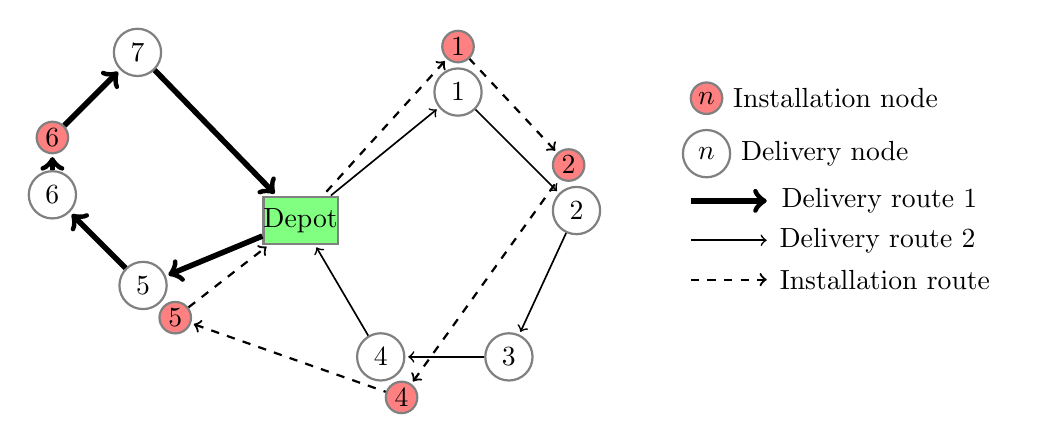
\begin{tikzpicture}
	[del/.style={circle,draw=black!50,thick, inner sep=0pt,minimum size=6mm},
	install/.style={circle,draw=black!50,fill=red!50,thick, inner sep=0pt,minimum size=4mm},
	depot/.style={rectangle,draw=black!50,fill=green!50,thick, inner sep=0pt,minimum size=6mm},
	pre/.style={<-,shorten <=1pt,thick,line width = 2pt },
	post/.style={->,shorten >=1pt,thick,line width = 2pt},
	pre1/.style={<-,shorten <=1pt,semithick},
	post1/.style={->,shorten >=1pt,semithick},
	pre2/.style={<-,shorten <=1pt,dashed,thick},
	post2/.style={->,shorten >=1pt,dashed,thick}]

	% first route
	\node [depot](Dpt) {Depot};
	\node [del] (d5) 	[below=2mm of Dpt,xshift=-20mm]{5}
		edge [pre] (Dpt);
	\node [del] (d6) 	[above left=10mm of d5]{6}
		edge [pre] (d5);
	\node [install] (i6) 	[above  =2.0mm of d6]{6}
	edge [pre] (d6);
	\node [del] (d7) 	[above right =10mm of i6]{7}
		edge [pre] (i6)
		edge [post] (Dpt);
	% Second route
	\node [del] (d1) 	[above=10mm of Dpt,xshift=20mm]{1}
		edge [pre1] (Dpt);
	\node [del] (d2) 	[below right=15mm of d1]{2}
		edge [pre1] (d1);
	\node [del] (d3) 	[below left =20mm of d2,xshift=10mm]{3}
	edge [pre1] (d2);
	\node [del] (d4) [left =10mm of d3]{4}
		edge [pre1] (d3)
		edge [post1] (Dpt);

	% Third route
	\node [install] (i1) 	[above=0.5mm of d1]{1}
		edge [pre2] (Dpt);
	\node [install] (i2) 	[above =.5mm of d2,xshift=-1mm]{2}
		edge [pre2] (i1);
	\node [install] (i4) 	[below right = 2mm of d4,xshift=-2.5mm]{4}
	edge [pre2] (i2);
	\node [install] (i5) [below right =0.5mm of d5]{5}
		edge [pre2] (i4)
		edge [post2] (Dpt);

		%Legende
	\node [install] (inode) 	[ below right=5mm of i1,xshift=25mm,label=right: Installation node ]{$n$} ;
	\node [del] (dnode) 	[below =5pt of inode,label=right: Delivery node]{$n$} ;
	\draw [post]($ (dnode) + (-0.2,-0.6) $) -- ($ (dnode) + (0.8,-0.6) $)
	node [right,align=center]
	 { Delivery route 1};
	 \draw [post1]($ (dnode) + (-.2,-1.1) $) -- ($ (dnode) + (0.8,-1.1) $)
	node [right,align=center]
	 { Delivery route 2 };
	 \draw [post2]($ (dnode) + (-.2,-1.6) $) -- ($ (dnode) + (0.8,-1.6) $)
	node [right,align=center]
	 { Installation route };
\end{tikzpicture}
\caption{Solution of a MCDIRP with seven customers}
\label{fig:fig1}
	\end{figure}
%\end{center}
\end{frame}

\section{Mathematical formulation}
\begin{frame}{}

\begin{block}{Variables}
		\begin{itemize}
	 		\item $x_{ijk}$  equal to 1 if a deliveryman travels from $i$ to $j$ using vehicle $k$, and 0 otherwise
	 		\item $y_{ijk}$ equal to 1 if an installer travels from $i$ to $j$ using vehicle $k$, and 0 otherwise 
	  		\item $z_{i}$ equal to 1 if a deliverymen installs at customer $i$ location, and 0 otherwise
	  	\end{itemize}
	\end{block}

	\begin{block}{Subsets}
		\begin{itemize}
	 		\item $D$ is the set of delivery nodes
	 		\item $I$ is the set of installation nodes
	 		\item  $D^I$ is the subset of delivery nodes that require an installation ($D^I \subseteq D$)
	  		\item $n(i)$ is the delivery node associated with the  installation node $i$
	  		\item  $l(j)$ is the installation node associated with the delivery node $j$
  		\end{itemize}
	\end{block}
	
\end{frame}
\begin{frame}[shrink=20]{Three-index formulation (1)}
\begin{figure}[]
 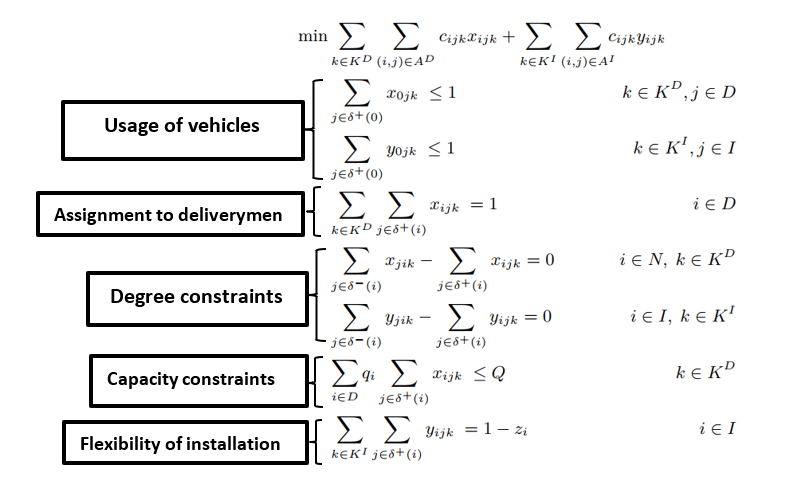
\includegraphics[scale=0.9]{equation1.PNG}
\end{figure}
\end{frame}

\begin{frame}[shrink=20]{Three-index formulation (2)}
\begin{figure}[]
 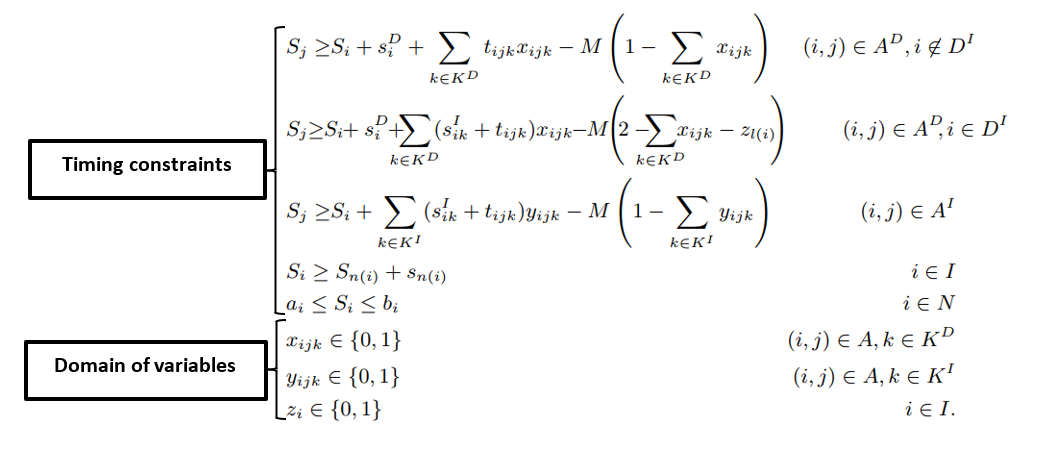
\includegraphics[scale=0.8]{equation2.PNG}
\end{figure}
\end{frame}

\iffalse
\begin{frame}[shrink=20]{Three-index formulation (1)}
\begin{align}
\label{model:obj} \min  &  \sum_{k \in K^{D}}\sum_{(i,j) \in A^D} c_{ijk}x_{ijk} + \sum_{k \in K^{I}}\sum_{(i,j) \in A^I} \hspace{-2mm}c_{ijk}y_{ijk} 
\end{align}
\begin{tcolorbox}[colback=red!5!white,colframe=red!75!black]
Usage of vehicles
\vspace{-2mm}
\end{tcolorbox}

\begin{align}
\label{c20} & \sum_{j \in \delta^{+}(0)}x_{0jk}\ \leq 1 & \hspace{-40mm}  k \in K^{D},j \in D \hspace{10mm}   \\
\label{c21} & \sum_{j \in \delta^{+}(0)}y_{0jk}\ \leq 1 & \hspace{-40mm}  k \in K^{I},j \in I \hspace{10mm} 
\end{align}
\begin{align}
\label{c22} & \sum_{k \in K^{D}}\sum_{j \in \delta^{+}(i)}x_{ijk}\ = 1 & \hspace{-40mm}   i \in D \hspace{10mm}  \\
\label{c23} & \sum_{j \in \delta^{-}(i)}x_{jik} - \sum_{j \in \delta^{+}(i)}x_{ijk} = 0 &\hspace{-40mm}   i \in N ,\ k \in K^{D} \hspace{10mm} \\
\label{c24} & \sum_{j \in \delta^{-}(i)}y_{jik} - \sum_{j \in \delta^{+}(i)}y_{ijk} = 0 & \hspace{-40mm}  i \in I ,\ k \in K^{I} \hspace{10mm}  \\
\label{c25} & \sum_{i \in D}q_{i} \sum_{j \in \delta^{+}(i)}x_{ijk}\ \leq Q & \hspace{-40mm}   k \in K^{D} \hspace{10mm}  \\
\label{c27} & \sum_{k \in K^{I}}\sum_{j \in \delta^{+}(i)}y_{ijk}\ = 1 - z_{i} & \hspace{-40mm}  i \in I \hspace{10mm}
\end{align}

\end{frame}

\begin{frame}[shrink=20]{Three-index formulation (2)}
\begin{align}
\label{c30} & S_j \geq \hspace{-1mm} S_i +  s_i^D + \sum_{k \in K^{D}} t_{ijk} x_{ijk} - M\left(1-\sum_{k \in K^{D}} x_{ijk}\right) & \hspace{-15mm}  (i,j) \in A^D, i \not\in D^I \hspace{7mm} \\
\label{c31} & S_j \hspace{-1mm} \geq \hspace{-1mm} S_i \hspace{-1mm}+ s^D_i \hspace{-1mm}+ \hspace{-3mm}\sum_{k \in K^{D}}\hspace{-1mm}(s_{ik}^I + t_{ijk} )x_{ijk} \hspace{-1mm}- \hspace{-1mm}M\hspace{-1mm}\left(\hspace{-1mm}2-\hspace{-3mm}\sum_{k \in K^{D}} \hspace{-2mm}x_{ijk}-z_{l(i)}\hspace{-1mm}\right)  &  \hspace{-4mm}   (i,j) \in A^D\hspace{-1mm}, i \in D^I \hspace{2mm}  \\
\label{c32} & S_j \geq \hspace{-1mm} S_i +  \sum_{k \in K^{I}}(s_{ik}^I + t_{ijk} )y_{ijk} - M\left(1-\sum_{k \in K^{I}} y_{ijk}\right)  & \hspace{-40mm}  (i,j) \in A^I \hspace{10mm} \\
\label{c33} & S_i \geq S_{n(i)} + s_{n(i)} & \hspace{-40mm}   i \in I \hspace{10mm}  \\
\label{c34}  & a_i \leq S_i \leq b_{i} & \hspace{-40mm}  i \in N \hspace{10mm} \\
\label{c36} & x_{ijk} \in \{0,1\} & \hspace{-50mm}  (i,j) \in A , k \in K^D  \hspace{10mm} \\
\label{c37} & y_{ijk} \in \{0,1\} & \hspace{-50mm} (i,j) \in A , k \in K^I  \hspace{10mm} \\
\label{c38} & z_{i} \in \{0,1\} & \hspace{-40mm}  i \in I. \hspace{10mm} 
\end{align}
\end{frame}
\fi

\section{ALNS algorithm}
\subsection{Operators}
\begin{frame}{ Adaptive Large Neighorhood Search}
	\begin{block}{First introduced in \citet{RopkePisinger} for the pickup and delivery routing problem}
	\begin{itemize}
			\item Initial solution
	 		\item {Destroy operators}
	 			\only<2>{
	 			\begin{itemize}
	 				\item Random delivery removal
			 		\item Related delivery removal	
	  			\end{itemize}
	  			}
	 		\item Repair operators	
	 		\only<2>{
	 			\begin{itemize}
	 				\item Greedy sequential insertion
			 		\item Regret-$k$ insertion
	  			\end{itemize}
	  			}
		\end{itemize}
	\end{block}

\end{frame}
\subsection{Preprocessing procedure}
\begin{frame}{Preprocessing procedure for insertion}
	\begin{block}{Forward time slack \citep{cordeau2004improved}}
		\begin{equation}
			\label{eq:slack1}
	 		F_i= \min_{i \leq k \leq \gamma+1}{ \sum_{i < p \leq k}{ W_{p} + (b_k-B_k)}\hspace{0.1cm}} 
	 	\end{equation}
	 	\begin{itemize}
	 		\item  $\gamma$: number of nodes in a route 
	 		\item $A_i$: arrival time at node $i$
	 		\item $B_i$: beginning service time at node $i$
	 		\item $W_{i}$: waiting time at node $i$
	 	\end{itemize}
	\end{block}		
	
	\begin{block}{Addition of the waiting time at node $i$}
		\begin{equation}
		\label{eq:slack}
	 F_i= \min_{i \leq k \leq \gamma+1}{ \sum_{i \leq p \leq k}{ W_{p} + (b_k-B_k)} \hspace{0.1cm} }
	 \end{equation}
	 $W_{i}= \max{\lbrace 0, a_{i} - A_{i} \rbrace} $ for a delivery node $i$ \\
	  $W_{l(i)}= \max{\lbrace 0, B_{i} + s_i - A_{l(i)} \rbrace} $ for its installation node $l(i)$
	 \end{block}	
\end{frame}

\begin{frame}{Preprocessing procedure for insertion}
\begin{block}{Delivery and installation on different routes}
		\begin{itemize}[]
	 		\item compute the arrival time at all delivery nodes of the route
			\item compute the arrival time at all installation nodes of the route
			\item compute $F_{l(i)}$ using equation~(\ref{eq:slack})
	 		\item compute $F_{i}$ as:
	  	\end{itemize}
	\begin{align*}		
	%\label{eq:slackdel}
	 \hspace{0mm} F_{i} = \min \left\lbrace  \hspace{-1mm} \min_{i < k \leq \gamma+1}{ \sum_{i < p \leq k}{ \hspace{-2mm}W_{p} + (b_k-B_k )}}, \hspace{1mm} b_i-B_i - s_i,\hspace{1mm} F_{l(i)}-W_{l(i)} \right\rbrace  + W_i  
	 \end{align*}
\end{block}
\end{frame}

\begin{frame}{Illustration of the forward time slack computation}
\begin{figure}[]
 \resizebox{1.1\linewidth}{!}{
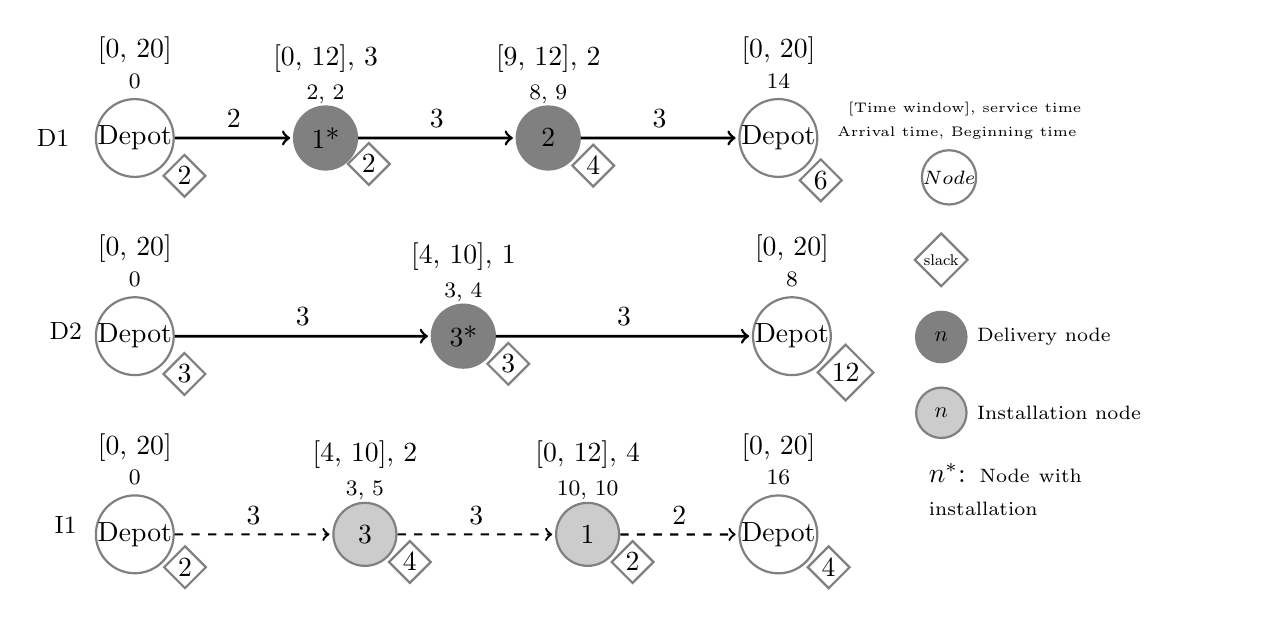
\begin{tikzpicture}
	[depot/.style={circle,draw=black!50,thick, inner sep=0pt,minimum size=6mm},
	install/.style={circle,draw=black!50,fill=black!20,thick, inner sep=0pt,minimum size=8mm},
	del/.style={circle,draw=black!50,fill=black!50,thick, inner sep=1pt,minimum size=8mm},
	st/.style={<->,shorten <=1pt,thick,line width = 1.5pt },
	pre/.style={<-,shorten <=1pt,thick,line width = 2pt },
	post/.style={->,shorten >=1pt,semithick,line width = 1.pt},
	pre1/.style={<-,shorten <=1pt,semithick},
	post1/.style={->,shorten >=1pt,semithick},
	pre2/.style={<-,shorten <=1pt,dashed,thick},
	post2/.style={->,shorten >=1pt,dashed,thick}
	,slack/.style={diamond,draw=black!50,thick, inner sep=1pt,minimum size=1mm}
	,strike/.style={strike out,draw=black!50,thick, inner sep=1pt,minimum size=1mm}, scale = 0.6
]
	% first route
	 \node (d1)[above= 0.mm,xshift= 0mm,yshift=-0mm]{ \small{D1}};
	 \node [depot](Dpt1) [right= 2 mm of d1,label={[xshift=.0cm, yshift=0.3cm][0, 20]},label={[xshift=.0cm, yshift=0.001cm] \footnotesize{0}}]{Depot};
	\node [slack](s1)[below right = 0.4mm of Dpt1,xshift=1mm,yshift=0.5mm]{2};
	%\node [strike](s1)[below left = 0.4mm of Dpt1,xshift=1mm,yshift=0.5mm]{5};
	\node [del] (d1) [right=15mm of Dpt1,label={[xshift=.0cm, yshift=0.3cm][0, 12], 3},label={[xshift=-.cm, yshift=-0.1cm] \footnotesize{2, 2}}]{1*};
	\node [slack](s2)[below right = 0.2mm of d1,xshift=1mm,yshift=1.2mm]{2};
	%\node [strike](s2)[below left = 0.2mm of d1,xshift=1mm,yshift=1.2mm]{5};
	 %\draw [st]($ (d1) + (-0.6,-0.75) $) -- ($ (d1) + (0.6,-0.75) $)
	 node [above= 0.mm,xshift= -5mm,yshift=-1.1mm]{ \scriptsize{1}};
		\path (Dpt1) edge[post]  node [ pos=0.5, sloped, above] {2} (d1);
	\node [del] (d2) [right =20mm of d1,label={[xshift=.0cm, yshift=0.3cm][9, 12], 2},label={[xshift=-.cm, yshift=-0.1cm] \footnotesize{8, 9}}]{2};
	\node [slack](s3)[below right = 0.5mm of d2,xshift=1mm,yshift=1.2mm]{4};
	 %\draw [st]($ (d2) + (-0.6,-0.75) $) -- ($ (d2) + (0.6,-0.75) $)
	 node [above= 0.mm,xshift= -5mm,yshift=-1.1mm]{ \scriptsize{1}};
	\path (d1) edge  [post] node [ pos=0.5, sloped, above] {3} (d2);
	\node [depot] (Dpt11) [ right =20mm of d2,label={[xshift=.0cm, yshift=0.3cm][0, 20]},label={[xshift=.0cm, yshift=0.001cm] \footnotesize{14}}]{Depot};
	\node [slack](s4)[below right = 0.5mm of Dpt11]{6};
	\path (d2) edge  [post] node [ pos=0.5, sloped, above] {3} (Dpt11);

	% 2nd road
	\node (d2)[below = 15 mm of d1,xshift= -33mm,yshift=-3mm]{ \small{D2}};
		\node [depot](Dpt2) [below= 15mm of Dpt1,label={[xshift=.0cm, yshift=0.3cm][0, 20]},label={[xshift=.0cm, yshift=0.001cm] \footnotesize{0}}]{Depot};
		\node [slack](s21)[below right = 0.4mm of Dpt2,xshift=1mm,yshift=0.5mm]{3};
		%\node [strike](s21)[below left = 0.4mm of Dpt2,xshift=1mm,yshift=0.5mm]{8};
	\node [del] (d3) [right=32.5mm of Dpt2,label={[xshift=.0cm, yshift=0.3cm][4, 10], 1},label={[xshift=-.cm, yshift=-0.1cm] \footnotesize{3, 4}}]{3*};
	\node [slack](s32)[below right = 0.5mm of d3,xshift=1mm,yshift=1.2mm]{3};
	%\node [strike](s32)[below left = 0.5mm of d3,xshift=1mm,yshift=1.2mm]{8};
	 %\draw [st]($ (d3) + (-0.6,-0.75) $) -- ($ (d3) + (0.6,-0.75) $)
	 node [above= 0.mm,xshift= -5mm,yshift=-1.mm]{ \scriptsize{1}};
		\path (Dpt2) edge[post]  node [ pos=0.5, sloped, above] {3} (d3);
	\node [depot] (Dpt22) [ right =32.5mm of d3,label={[xshift=.0cm, yshift=0.3cm][0, 20]},label={[xshift=.0cm, yshift=0.001cm] \footnotesize{8}}]{Depot};
	\node [slack](s322)[below right = 0.5mm of Dpt22,xshift=1mm,yshift=1.2mm]{12};
	\path (d3) edge  [post] node [ pos=0.5, sloped, above] {3} (Dpt22);

	%3rd road (installer)
		\node (I1)[below = 15 mm of d2,xshift= -0mm,yshift=-5mm]{ \small{I1}};
		\node [depot](Dpt3) [below= 15 mm of Dpt2,label={[xshift=.0cm, yshift=0.3cm][0, 20]},label={[xshift=.0cm, yshift=0.001cm] \footnotesize{0}}]{Depot};
		\node [slack](sDpt3)[below right = 0.5mm of Dpt3,xshift=1mm,yshift=1.2mm]{2};
	\node [install] (i1) [right=20mm of Dpt3,label={[xshift=.0cm, yshift=0.3cm][4, 10], 2},label={[xshift=-.0cm, yshift=-0.1cm] \footnotesize{3, 5}}]{3};
	\node [slack](si1)[below right = 0.5mm of i1,xshift=1mm,yshift=1.2mm]{4};
	 %\draw [st]($ (i1) + (-0.6,-0.75) $) -- ($ (i1) + (0.6,-0.75) $)
	 node [above= 0.mm,xshift= -5mm,yshift=-1.1mm]{ \scriptsize{2}};
		\path (Dpt3) edge[post2]  node [ pos=0.5, sloped, above] {3} (i1);

	\node [install] (i3) [right =20mm of i1,label={[xshift=.0cm, yshift=0.3cm][0, 12], 4},label={[xshift=-.0cm, yshift=-0.1cm] \footnotesize{10, 10}}]{1};
	\node [slack](si3)[below right = 0.5mm of i3,xshift=1mm,yshift=1.2mm]{2};
	% \draw [st]($ (i3) + (-0.6,-0.75) $) -- ($ (i3) + (0.6,-0.75) $)
	 node [above= 0.mm,xshift= -5mm,yshift=-1.1mm]{ \scriptsize{1}};
	\path (i1) edge  [post2] node [ pos=0.5, sloped, above] {3} (i3);
	\node [depot] (Dpt31) [ right =15mm of i3,label={[xshift=.0cm, yshift=0.3cm][0, 20]},label={[xshift=.0cm, yshift=0.001cm] \footnotesize{16}}]{Depot};
	\node [slack](sDpt31)[below right = 0.5mm of Dpt31,xshift=1mm,yshift=1.2mm]{4};
	\path (i3) edge  [post2] node [ pos=0.5, sloped, above] {2} (Dpt31);

		%Legende

	 \node [depot] (inode) [  right =15mm of Dpt11,xshift=-02mm,yshift=-5mm,label={[xshift=2mm, yshift=0.3cm]\tiny{[Time window], service time}},label={[xshift=1mm, yshift=0.001cm] \tiny{Arrival time, Beginning time}}]{\scriptsize{$Node$}} ;
	  %\draw [st]($ (inode) + (-0.5,-0.6) $) -- ($ (inode) + (0.5,-0.6) $)
	 node [above= 0.mm,xshift= -5mm,yshift=-0.5mm]{ \tiny{Service time}};
	 \node [slack](slack)[below  = 3.5mm of inode,xshift=-1mm,yshift=0.1mm,scale=0.7]{\footnotesize{slack}};
	 %\node [strike](sinode)[below  = 2mm of slack,xshift=-1mm,yshift=0.1mm,scale=0.8,label=right: \small{Wrong value of slack} $n$]{\footnotesize{Slack}};
	 \node [del] (dnode) [below =3 mm of slack,scale=0.8,label=right: \scriptsize{Delivery node }]{$n$} ;
	 \node [install] (insnode) [below =3 mm of dnode,scale=0.8,label=right: \scriptsize{Installation node}]{$n$} ;
	  \node  (n) [below right =4mm of insnode,text width=4cm,xshift= -0.8cm,scale=1]{$n^*$: \scriptsize{Node with \\ installation}} ;
	% \draw [post]($ (dnode) + (-0.2,-0.6) $) -- ($ (dnode) + (0.8,-0.6) $)
\end{tikzpicture}}
%\caption{Computation of the forward time slacks}
\label{fig:slack}
	\end{figure}
%\end{center}
\end{frame}

\section{Computational experiments}

\subsection{Instances}
\begin{frame}{Instances generation}
\begin{block}{Modification of Solomon instances \citep{Solomon1987} for the  VRPTW}
 \begin{itemize}
	 \setlength{\parskip}{0pt} 
 	\setlength{\itemsep}{0pt plus 1pt}
	 \item Customers: 15, 25, 50, 100
	 \item Speeds of each delivery/installation vehicle: 1/2
	 \item Costs of the delivery/installation vehicles: 2/1, 5/1 and 10/1
	 \item Efficiency of the deliverymen when installing: [30\%, 50\%], [60\%, 80\%]
	 \item Percentage of customers with installation: 20\%, 50\% and 75\%
 \end{itemize} 
\end{block}
\end{frame}

\subsection{Parameters tuning}

\begin{frame}{ALNS parameters tuning}
\begin{block}{Number of iterations}
	\begin{figure}[]
		
		\label{fig:fig2}
			\pgfplotsset{every tick label/.append style={font=\tiny},width=7.15cm,compat=1.15}
			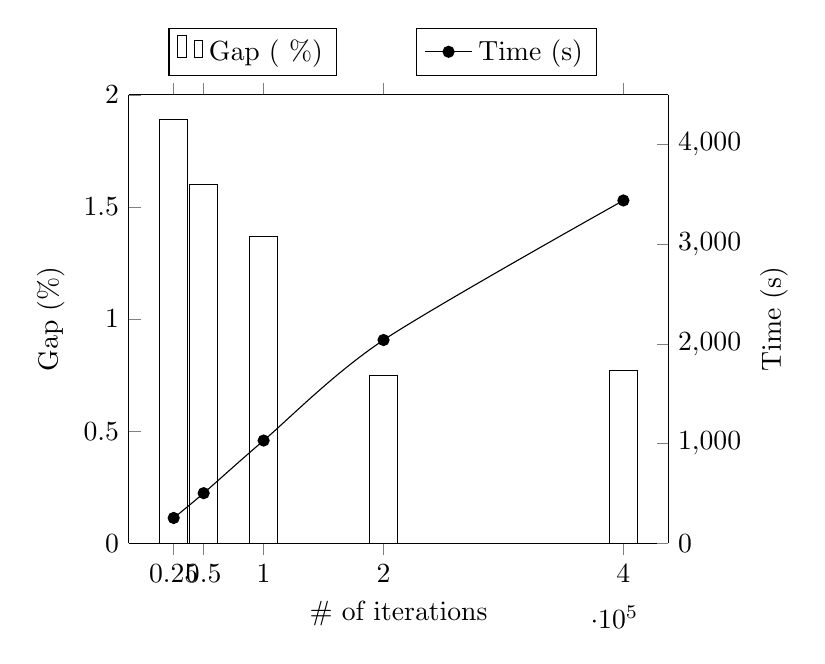
\begin{tikzpicture}

			\begin{axis}[
				%x tick label style={
			%rotate = 90,
			%/pgf/number format/1000 sep=},
			%symbolic x coords={25000,50000,100000,200000,400000},
    			xtick=data,
			ylabel=Gap (\%),
			%enlargelimits=0.1,
			legend style={at={(0.23,1.15)},
			anchor=north,legend columns=1},
			ybar,
			%ybar = 15pt,	
			bar width=10pt,
			axis y line*=left,
  			ymin=0, ymax=2,
 			xlabel= \# of iterations,
			%enlargelimits=true
			%enlarge x limits=false, try min ticks={10} 
		]
		\addplot[black]   coordinates{
		(25000,	1.89)
		(50000,	1.6)
		(100000,1.37)
		(200000, 0.75)
		(400000	, 0.77)
		};
		\legend{Gap ( \%)}
	\end{axis}
	\begin{axis}[
  		axis y line*=right,
		  axis x line=none,
		  ymin=0	, ymax=4500,
		  ylabel= Time (s),
			legend style={at={(0.7,1.15)},
		anchor=north,legend columns=-1},
		%nodes near coords
		]

		\addplot[smooth,mark=*,]
		  coordinates{
			(25000,	253.61)
			(50000,	502.55)
			(100000, 1030.79)
			(200000, 2039.79)
			(400000	, 3440.62)
			};
		 \legend{Time (s)}

	\end{axis}

	\end{tikzpicture}
	%\caption{Effect of the number of iterations on the performance of the ALNS}
	\end{figure}
	\end{block}
\end{frame}

\iffalse
\begin{frame}{ALNS parameters tuning}
	\begin{block}{Operators available}
	\begin{itemize}
 \setlength{\parskip}{0pt} 
 \setlength{\itemsep}{0pt plus 1pt}
	\item Destroy operators: random and related removal
	\item Repair operators: greedy sequential (seq), regret-$3$, regret-$m$, regret-$3n$, regret-$mn$
\end{itemize}
	\end{block}
	\begin{block}{Operators selected within  $2^{7}$ combinations}
	\begin{itemize}
 \setlength{\parskip}{0pt} 
 \setlength{\itemsep}{0pt plus 1pt}
	\item Apply a resolution $III$ fractional factorial design on the five repair heuristics to reduce the number of combinations to $2^{3}$ from $2^5$
	\item Add one of the removal operators to each combination of insertion operators
	\item  Add to each combination of insertion operators the two available removal operators
\end{itemize}
\end{block}
\end{frame}
\fi

\begin{frame}{ALNS parameters tuning}
	\begin{block}{Operators available}
		\begin{itemize}
 \setlength{\parskip}{0pt} 
 \setlength{\itemsep}{0pt plus 1pt}
			\item Destroy operators: random and related removal
			\item Repair operators: greedy sequential (seq), regret-$3$, regret-$m$, regret-$3n$, regret-$mn$
		\end{itemize}
	\end{block}
	
\end{frame}

\begin{frame}<1>[label=zooms]
\frametitle{{Operators selection}}

\fontfamily{lmss}\selectfont{
	\begin{table}[]
\caption{\small{Quality of the solution when combining the operators}}
\vspace*{-2mm}
\label{tab:combo1}
\resizebox{\textwidth}{!}{
\begin{tabular}{|l|c|c|c|}
\hline
\textbf{Combination of operators}    & \textbf{Gap (\%)} & \textbf{Time  (s)} & \textbf{\% of improvement} \\ \hline
seq, regret-3, regret-$m$, regret-3$n$, regret-$$mn$$, related       & -1.20 & 643.7             & 86.9                      \\ \hline
seq, regret-3, regret-$m$, regret-$3n$, regret-$mn$, random, related & -1.08             & 648.5             & 85.2                      \\ \hline
seq, regret-$m$, regret-$mn$, random                                 & -0.98             & 690.6             & 84.3                      \\ \hline
seq, regret-3, regret-$m$, regret-$3n$, regret-$mn$, random & -0.96 & 649.5   & 83.5 \\ \hline
seq, regret-$m$, regret-$mn$, random, related                        & -1.10              & 680.8             & 82.6                  \\ \hline
seq, regret-3, regret-$3n$, related  & -0.62 & 531.1 & 82.6                      \\ \hline
seq, regret-$m$, regret-$mn$, related                                & -0.96             & 667.4             & 80.9                      \\ \hline
seq, regret-3, regret-$3n$, random, related                          & -0.59             & 535.9             & 79.1                      \\ \hline
regret-3, regret-$mn$, related                                       & -0.80              & 708.4             & 78.3                      \\ \hline
regret-3, regret-$m$, related                                        & -0.80              & 708.6             & 78.2                      \\ \hline
regret-$3n$, regret-$mn$, related                                    & -0.80              & 712.2              & 78.3                      \\ \hline
seq, random   & -0.36             & 132.3             & 78.3                      \\ \hline
seq, related         & -0.35             & 131.1             & 78.3                     \\ \hline
seq, regret-3, regret-$3n$, random                                   & -0.49             & 534.2             & 77.4                      \\ \hline
regret-$m$, regret-$3n$, related  & -0.71             & 707.8             & 75.6                      \\ \hline
regret-3, regret-$mn$, random                                        & -0.61             & 727.5             & 75.6                      \\ \hline
regret-3, regret-$m$, random  & -0.60              & 732.0                & 75.6                      \\ \hline
regret-3, regret-$m$, random, related    & -0.82             & 711.8             & 74.8                     \\ \hline
regret-$3n$, regret-$mn$, random, related                            & -0.82             & 712.6              & 74.8                      \\ \hline
regret-3, regret-$mn$, random, related     & -0.82             & 714.8             & 74.8                      \\ \hline
regret-$3n$, regret-$mn$, random   & -0.58             & 737.2             & 74.8                      \\ \hline
regret-$m$, regret-$3n$, random   & -0.87             & 728.5             & 73.9                      \\ \hline
regret-$m$, regret-$3n$, random, related                             & -0.80              & 720.2             & 73.9                      \\ \hline
seq, random, related                                                 & -0.54             & 133.4              & 73.9   \\ \hline 
\end{tabular} }
\end{table}
}
\end{frame}

\subsection{Results}

\begin{frame}{Results}
\fontfamily{lmss}\selectfont{
\begin{table}[]
\centering
\caption{Results for all instances}
\label{alns1}
\resizebox{\textwidth}{!}{%
\begin{tabular}{@{}p{0.7cm}lp{0.9cm}p{0.9cm}llclp{0.9cm}p{0.9cm}llcl@{}}
\hline
\multicolumn{1}{l}{} &  & \multicolumn{6}{c}{{[}30\%, 50\%{]}} & \multicolumn{6}{c}{{[}60\%, 80\%{]}} \\ \cmidrule(l){3-8} \cmidrule(l){9-14}
Del cost & \%Inst & Best(\%) & Avg(\%) & Del & Inst & Time(s) & Gap & Best(\%) & Avg(\%) & Del & Inst & Time(s) & Gap \\
\hline
\\[-1em]
\multirow{3}{*}{2} & 20\% & 0.0 & 0.2 & 3.3 & 0.2 & 51.3 & 16.5 & 0.0 & 0.2 & 3.2 & 0.1 & 51.7 & 15.6 \\
 & 50\% & 0.1 & 0.4 & 3.5 & 0.4 & 126.8 & 19.5 & 0.0 & 0.2 & 3.5 & 0.2 & 128.7 & 18.5 \\
 & 75\% & 0.0 & 0.4 & 3.8 & 0.6 & 190.2 & 22.6 & 0.0 & 0.4 & 3.7 & 0.3 & 190.2 & 21.3 \\[0.5em]
\multirow{3}{*}{5} & 20\% & 0.0 & 0.2 & 3.3 & 0.3 & 50.5 & 16.6 & 0.0 & 0.2 & 3.2 & 0.2 & 52.4 & 15.7 \\
 & 50\% & 0.0 & 0.3 & 3.4 & 0.6 & 128.5 & 19.3 & 0.0 & 0.3 & 3.3 & 0.4 & 129.1 & 19.0 \\
 & 75\% & 0.0 & 0.4 & 3.5 & 0.9 & 200.3 & 21.6 & 0.0 & 0.5 & 3.5 & 0.7 & 203.4 & 21.5 \\[0.5em]
\multirow{3}{*}{10} & 20\% & 0.0 & 0.2 & 3.2 & 0.4 & 51.0 & 17.1 & 0.0 & 0.2 & 3.1 & 0.2 & 52.5 & 16.0 \\
 & 50\% & 0.0 & 0.3 & 3.3 & 0.9 & 131.2 & 18.9 & 0.0 & 0.2 & 3.2 & 0.6 & 127.4 & 18.5 \\
 & 75\% & 0.0 & 0.4 & 3.4 & 1.3 & 200.7 & 21.2 & 0.0 & 0.4 & 3.3 & 0.9 & 197.2 & 21.0 \\
 \cmidrule{1-14}
\multicolumn{2}{c}{Average} & 0.0 & 0.3 & 3.4 & 0.6 & 125.6 & 19.2 & 0.0 & 0.3 & 3.3 & 0.4 & 125.8 & 18.6 \\ \bottomrule
\end{tabular}%
}
\end{table}
}
\end{frame}

\begin{frame}{Results}

\fontfamily{lmss}\selectfont{
\begin{table}[]
\centering
\caption{Results for all optimal instances}
\label{tab:my-table}
\resizebox{1.\textwidth}{!}{%
 \begin{tabular}{@{}cp{1.68cm}|cccc|cccc|cccc@{}}
	\cmidrule(r){3-14} &  & \multicolumn{4}{c|}{2}            & \multicolumn{4}{c|}{5}& \multicolumn{4}{c}{10}\\
\hline
\% of inst & \multicolumn{1}{c|}{Perf} & Opt & Best (\%) & Time & Gap & Opt & Best (\%) & Time & Gap & Opt & Best (\%) & Time & Gap \\
\hline
\multirow{2}{*}{20} & {[}30\%, 50\%{]} & 30    & 0.1 & 9    & 37  & 29    & 0.1 & 5.9  & 37.6        & 26    & 0.1 & 8.5  & 36.7        \\
  & {[}60\%, 80\%{]} & 30    & 0.1 & 5.3  & 33.7        & 30    & 0.0   & 9.6  & 34.7        & 28    & 0.0   & 8.8  & 34.6        \\
 \hline
\multirow{2}{*}{50} & {[}30\%, 50\%{]} & 27    & 0.2 & 10   & 43.8        & 24    & 0.2 & 13.9 & 41.8        & 22    & 0.1 & 13.5 & 39.2        \\
                    & {[}60\%, 80\%{]} & 25    & 0.1 & 8.1  & 39.2        & 21    & 0.2 & 7.2  & 38.8        & 23    & 0.1 & 8.4  & 39          \\
                        \hline
\multirow{2}{*}{75} & {[}30\%, 50\%{]} & 18    & 0.0   & 13.4 & 45.1        & 18    & 0.0   & 14.5 & 43.5        & 16    & 0.0   & 24.6 & 41.1        \\
                    & {[}60\%, 80\%{]} & 22    & 0.0   & 14.5 & 44.5        & 17    & 0.0   & 11.2 & 43          & 18    & 0.0   & 13.2 & 42.4        \\
                    \hline
 \multicolumn{2}{c|} {Solved}           & \multicolumn{4}{c|}{152}          & \multicolumn{4}{c|}{139}          & \multicolumn{4}{c}{133}       \\
 \bottomrule 
\end{tabular}%
}
\end{table}
}
\end{frame}

\iffalse
\begin{frame}{Flexibility of the mathematical model}
\vspace*{-5mm}
	
\begin{block}{ } 
	 \begin{itemize}[]
	 	\item $z_i$ = 0
	 		\begin{itemize}
				\item Installation made only by installers	
				\item Equivalent to the VRPMS of \cite{HOJABRI201887}
			\end{itemize}
		\item $z_i$ = 1
			\begin{itemize}
		 		\item Installation made by deliverymen
				\item Equivalent to the VRPTWDST of \cite{schneider2016vehicle}
			\end{itemize}
	\end{itemize}
\end{block}
	
\end{frame}
\fi
\begin{frame}{Results}
\vspace*{-2mm}
 \[ \sum_{k \in K^{I}}\sum_{j \in \delta^{+}(i)}y_{ijk}\ = \only<1>{1 - z_{i}} \only<2>{0} \only<3>{1} \only<4>{1 - z_{i}}  \hspace{10mm} i \in I \hspace{3mm} \only<2>{\text{\alert{Deliverymen make all installations}}} \only<3>{\text{\alert{Deliverymen never install}}} \only<4>{\text{\alert{Both can install}}}\]
   
\fontfamily{lmss}\selectfont{

 Comparison when deliverymen efficiency are within {[}30\%, 50\%{]}

	\begin{table}[!htbp]
\centering
\vspace*{-3mm}
\label{bus_set1}
\resizebox{\textwidth}{!} & \multicolumn{4}{c}{50\%} & \multicolumn{4}{c}{75\%} \\ \cmidrule(l){2-5} \cmidrule(l){6-9} \cmidrule(l){10-13}
Del cost &  Opt & $z_i=1$ & $z_i=0$ & \small DIRPTW & Opt& $z_i=1$ & $z_i=0$ & \small DIRPTW &  Opt& $z_i=1$ & $z_i=0$ & \small DIRPTW \\
\hline
\\[-0.8em]
  \multicolumn{1}{l}{2} &28 &909.6 & 908.6 & \textbf{864.2} &26 &722.6 & 803.3 & \textbf{696.1} &17& 896.1 & 1106.9 & \textbf{855.2} \\[0.3em]
  
 \multicolumn{1}{l}{5} &29& 2247.8 & 2014.7 & \textbf{1972.4} & 24&2481.6 & 2107.0 & \textbf{2020.0} &28& 2107.9 & 1860.2 & \textbf{1709.8} \\[0.3em]
 
 \multicolumn{1}{l}{10} &26& 4507.6 & 3875.3 & \textbf{3838.4}& 22& 5008.6 & 3985.3 & \textbf{3899.5} &16& 5887.6 & 4174.9 & \textbf{4051.2} \\ \bottomrule
\end{tabular}%
}
\end{table}
}
Comparison when deliverymen efficiency are within {[}60\%, 80\%{]}
\fontfamily{lmss}\selectfont{
	\begin{table}[!htbp]
\centering
\vspace*{-3mm}
\label{bus_set2}
\resizebox{\textwidth}{!} & \multicolumn{4}{c}{50\%} & \multicolumn{4}{c}{75\%} \\ \cmidrule(l){2-5} \cmidrule(l){6-9} \cmidrule(l){10-13}
Del cost &  Opt & $z_i=1$ & $z_i=0$ & \small DIRPTW & Opt& $z_i=1$ & $z_i=0$ & \small DIRPTW &  Opt& $z_i=1$ & $z_i=0$ & \small DIRPTW \\
\hline
\\[-0.8em]
\multicolumn{1}{l}{2} &27& {635.0} & 719.9 & \textbf{633.4} &24& \textbf{619.6} & 794.6 & 640.3 &21 &\textbf{913.2} & 1268.8 & 920.7 \\[0.3em]
\multicolumn{1}{l}{5} &30 &2256.3 & 2275.2 & \textbf{2182.8} &21& 1589.9 & 1724.3 & \textbf{1574.6} & 17&1446.8 & 1630.2 & \textbf{1424.9} \\[0.3em]
\multicolumn{1}{l}{10} &28& 4066.8 & 3868.1 & \textbf{3795.7} &23& 3052.3 & 3112.8 & \textbf{2972.6} &18&3429.5 & 3299.0 & \textbf{3182.9} \\ \bottomrule
\end{tabular}%
}
\end{table}
}

\end{frame}

\begin{frame}{Managerial insights}
\begin{block}{}
	\begin{itemize}
		\item The proposed strategy is better than the traditional strategies 
		\item  No need for installation fleet in the following cases: 
			\begin{itemize}
				\item A small number of customers with very few having an installation regardless of the cost or the performance of the deliveryman 
				\item Low deliveryman cost, higher efficiency, medium size of customers
			\end{itemize}
		\item Use a distinct installation fleet is better when:
			\begin{itemize}
				\item[•] Deliverymen efficiency are low and the cost range from medium to high
				\item Deliverymen efficiency and cost are both high
			\end{itemize}
	\end{itemize}
\end{block}{}
\end{frame}

\begin{frame}[allowframebreaks]{Performance on the VRPMS instances set}
	\begin{block}{ \cite{HOJABRI201887} studied the delivery and installation of large items}
		\begin{itemize}
			\item Two distinct fleets are used
			\item A deliveryman and its installer arrival must be synchronized at a certain number of customer locations
			\item The installer must visit the customer within \textbf{ten} units of time after the start of the delivery service
		\end{itemize}
	\end{block}

\end{frame}

\begin{frame}{Results on the VRPMS instances set}
\fontfamily{lmss}\selectfont{
\textbf{Performance on the VRPMS instances}
\begin{table}[]
	%\caption{\small Performance on the VRPMS instances}
	\label{vrpms}
\resizebox{0.95\textwidth}{!}{
	\begin{tabular}{@{}cccccccccc}
	\toprule
	\multicolumn{1}{c}{} & \multicolumn{4}{c}{\cite{HOJABRI201887}}                                                    & \multicolumn{5}{c}{ALNS}  \\
 \cmidrule(l){2-5}   \cmidrule(l){6-10}
& \multirow{1}{*}{Best(\%)} & \multirow{1}{*}{Del}     & \multirow{1}{*}{Inst}    & \multirow{1}{*}{   Time (s)}       & Best(\%) & Avg (\%) & \multirow{1}{*}{Del} & \multirow{1}{*}{Inst} & \multirow{1}{*}{Time (s)} \\
\hline
\\[-1em] 
 \multicolumn{1}{r}{Average}     & \multicolumn{1}{c}{6.9}  & \multicolumn{1}{c}{8.4}  & \multicolumn{1}{c}{3.7} & \multicolumn{1}{c}{63681.0}   & \multicolumn{1}{c}{0.0}  & \multicolumn{1}{c}{0.3} & \multicolumn{1}{c}{7.6} & \multicolumn{1}{c}{3.4} & \multicolumn{1}{c}{170.7} \\
                  \hline
\end{tabular}}
\end{table}

\pause
%\begin{frame}{Results on the VRPMS instances set}

\textbf{Results for instances solved optimally with CPLEX}
\begin{table}[H]
%\caption{\small Results for instances solved optimally on VRPMS instances set}
\vspace*{-1mm}
\label{vrpmsExact}
\resizebox{1\textwidth}{!}{
\begin{tabular}{m{0.4cm}|cccccccccccccc}
\toprule
\multicolumn{1}{l}{}   & \multicolumn{4}{c}{\cite{HOJABRI201887}} & \multicolumn{5}{c}{ALNS}                                                                                                                       & \multicolumn{5}{c}{Exact method}                                                                                               \\ \cmidrule(r){2-5}\cmidrule(r){6-10}\cmidrule(r){11-15}
%\small
\multirow{1}{*}{} & \multirow{1}{*}{\small {Best (\%)}} & \multirow{1}{*}{Del}     & \multirow{1}{*}{Inst}    & \multirow{1}{*}{Time (s)}       & \multicolumn{1}{c}{Best (\%)}   & Avg (\%) & \multirow{1}{*}{Del} & \multirow{1}{*}{Inst} & \multicolumn{1}{c}{\multirow{1}{*}{Time (s)}} & \multicolumn{1}{c}{\multirow{1}{*}{Opt}} & \multirow{1}{*}{\small{Gap(\%) }} & \multirow{1}{*}{Del} & \multirow{1}{*}{Inst} & \multirow{1}{*}{Time (s)}   \\ \cline{1-15} 
 
\\[-0.8em]            
\multicolumn{1}{r}{Average}  & 3.0  & 9.1  & 4.3   & 33319.8  & 0.2    & 0.3  & 8.5 & 4.1 & 72.7 & 20.3 & 34.2  & 8.5   & 4.1   & 505.7   \\ \hline         
\multicolumn{1}{r|}{Solved}  &\multicolumn{4}{c}{44} &\multicolumn{5}{c}{122}  & \multicolumn{5}{c}{139}  \\ \hline         
\end{tabular}}
\end{table}
}
\end{frame}

\begin{frame}[allowframebreaks]{Performance on the VRPTWDST instances set}
\vspace*{10mm}
	\begin{block}{ \cite{schneider2016vehicle} }
		\begin{itemize}
			\item Drivers have different efficiency with their customers
			\item Drivers have specific travel and service times in order to model their familiarity with the customers to visit
			\item No synchronization constraints
		\end{itemize}
	\end{block}

%\end{frame}
%\begin{frame}[allowframebreaks]{Results on the VRPTWDST instances set}
\newpage
\vspace*{-5mm}
\fontfamily{lmss}\selectfont{

\vspace*{-5mm}


\begin{table}[]
\centering
\caption{Lower and upper bounds for the VRPTWDST for the secondary objective of minimizing travelled distance}
\label{tab:random}
\resizebox{0.8\textwidth}{!}{%
\begin{tabular}{lcllcllll}
\toprule
  & \multicolumn{3}{c}{ \cite{schneider2016vehicle}}
  & \multicolumn{3}{c}{ALNS} & \multicolumn{2}{c}{Exact} \\
 \cmidrule(l){2-4} \cmidrule(l){5-7} \cmidrule(l){8-9}
  & Best (\%) & Opt & Time & Best (\%)& Opt & Time &  Gap(\%)& Opt \\
\hline
  C1 & 0.0 & 28/90 & 6.9 & 0.0 & 28/90 & 33.7 & 22.0 & 28/90 \\
 C2 & 0.0 & 24/80 & 10.5 & 0.0 & 24/80 & 46.8 & 4.1 & 24/80 \\
 R1 & 2.4 & 0/120 & 94.7 & 0.2 & 4/120 & 37.6 & 28.7 & 8/120 \\
 R2 & 6.6 & 0/110 & 45.3 & 0.1 & 0/110 & 73.2 & 19.6 & 0/110 \\
 RC1 & 3.8 & 0/80 & 53.1 & 0.3 & 0/80 & 32.6 & 40.2 & 0/80 \\
 RC2 & 10.7 & 0/80 & 67.4 & 0.1 & 0/80 & 54.1 & 28.6 & 0/80 \\[0.5em]
\hline
\multicolumn{1}{l}{Average} & 3.9 & - & 52.8 & 0.1 & - & 46.9 & 24.0 & - \\
 \hline
\multicolumn{1}{l}{Solved} & \multicolumn{3}{c}{52/560} &\multicolumn{3}{c}{56/560} &\multicolumn{2}{c}{60/560} \\
\hline
\end{tabular}%
}
\end{table}}

\end{frame}


\section{Conclusion}
\begin{frame}{Conclusion}

	\begin{itemize}
		\item Novel distribution strategy proposed
		\item Insights about existing distribution and installation strategies
		\item An exact and heuristic algorithm to solve the DIRPTW
		\item New best-know and optimal solutions for the VRPMS and the VRPTWDST
	\end{itemize}
	\begin{block}{Applications of the DIRPTW}
		Choose between a specialist and a generalist in the home care staff scheduling problem
	\end{block}
\end{frame}

\appendix

\begin{frame}[allowframebreaks]{References}

  \bibliography{biblio}
  \bibliographystyle{plainnat}

\end{frame}

\end{document}
